%!TEX root =  main.tex

\section{RamCast: RDMA-based Atomic Multicast}
\label{sec:rdma-atomic-multicast}

In this section, we recall the building blocks that inspired \libname (\S\ref{sec:bblocks}) and present its design and algorithms. 
We start with an overview of \libname (\S\ref{sec:overview}), then detail its data structures (\S\ref{sec:ds-structs}) and algorithms in the absence of failures (\S\ref{sec:normalcase}) and in the presence of failures (\S\ref{sec:failurecase}).
We conclude with a few extensions to the protocol (\S\ref{sec:extensions}).
We argue for the correctness of \libname in the Appendix.\footnote{https://www.dropbox.com/s/nlwzujxrtz5eopj/ramcast-proof.pdf?dl=0}

\subsection{Building blocks}
\label{sec:bblocks}

\libname leverages two ideas, Skeen's atomic multicast algorithm \cite{BJ87b} and Protected Memory Paxos \cite{Aguilera2019}.
Skeen's algorithm orders messages multicast to multiple processes consistently but it does not tolerate failures.
Protected Memory Paxos takes advantage of RDMA permissions to improve the efficiency of Paxos \cite{L98}. 
Like Paxos, it implements atomic broadcast (i.e., it assumes a single group of processes).
%Combining these ideas coherently and efficiently is not trivial, as we discuss in this section,
%after briefly presenting Skeen's algorithm and Protected Memory Paxos.

%\subsubsection{Skeen's atomic multicast}

\subsubsection{Skeen's atomic multicast}

In Skeen's algorithm, each process assigns unique timestamps to multicast messages based on a logical clock~\cite{Lam78}.
The correctness of the algorithm stems from two basic properties:
(i)~processes in the destination of a multicast message first assign tentative timestamps to the message and eventually agree on the message's final timestamp; and
(ii)~processes deliver messages according to their final timestamp.
These properties are implemented as follows.

\begin{itemize}
\item[(i)] To multicast a message $m$ to a set of processes, $p$ sends $m$ to the destinations.
Upon receiving $m$, each destination updates its logical clock, assigns a tentative timestamp to $m$, stores $m$ and its timestamp in a buffer, and sends $m$'s timestamp to all destinations.
Upon receiving timestamps from all destinations in $m.dst$, a process computes $m$'s final timestamp as the maximum among all received tentative timestamps for $m$.
\item[(ii)]Messages are delivered respecting the order of their final timestamp.
A process $p$ delivers $m$ when it can ascertain that $m$'s final timestamp is smaller than the final timestamp of any messages $p$ will deliver after $m$ (intuitively, this holds because logical clocks are monotonically increasing).
\end{itemize}

\subsubsection{Protected Memory Paxos}
\label{sec:PMP}

In Paxos \cite{L98}, to order a message $m$, the leader proposes $m$ in a consensus instance.
In the normal case, where there is a single leader, the followers accept the proposed message and reply to the leader.
In Protected Memory Paxos, the followers grant exclusive write permission to their memory to the leader.
If a new leader takes over, then it revokes the permission of the previous leader.
To order $m$, the leader writes $m$ in the memory of the followers.
If the leader succeeds in writing the message in the memory of a quorum of followers, then no other leader took over, and the message is ordered.

Just like Paxos, to ensure that the new leader makes decisions that are consistent with the decisions of the previous leader, each leader associates a \emph{round} to its proposed message.
%A round is a tuple $\langle rnd, pid \rangle$, where $rnd$ is a scalar and $pid$ is the process unique identifier, used to make rounds unique across the system.
Rounds are unique across the system.
%The very first leader, say process $p$, uses round $\langle 0, p \rangle$.
When process $q$ becomes leader, upon suspecting the failure of the current leader $p$, $q$ must pick a round bigger than $p$'s round.
Process $q$ then proceeds in two steps.
First, $q$ needs to acquire permission from a quorum of processes, which it does by contacting all processes and providing its chosen round.
Processes grant write permission to $q$ if the provided round is bigger than the round of the process that currently holds the write permission.
Second, $q$ must check whether other processes have already accepted any values.
If so, $q$ must propose the value that has been accepted in the largest round; otherwise, $q$ can propose a new value.

\subsection{\libname design and architecture}
\label{sec:overview}

Figure~\ref{fig:arch} depicts the various components and memory layout of \libname.
Processes within each group coordinate using the leader-follower model \cite{gotsman2019white,Junqueira2011,Mu,delta4}.
Each server process has a fixed-size buffer per client, analogously to other RDMA-based systems \cite{FaRM, Mu, DARE, APUS}.
A buffer in \libname is divided into two parts, a message buffer $M$, and a timestamp buffer $T$.
Message buffer $M$ is a shared memory region that can be read and written by any processes, including the client process the buffer is associated with.
Timestamp buffer $T$ is protected and can only be written by the leader of each group; the buffer can be read by any processes.
Each slot in $M$, with a multicast message $m$, has a corresponding slot in $T$, with $m$'s timestamp.

%Each server process organizes its memory in regions: a shared
%memory region and a protected memory region. All processes have remote access
%(read/write) to the shared memory space. 
%Only one leader of each group
%has remote-write permission to a given node's log at any point in time
%during the protocol.

Clients keep a copy of the remote head and tail pointer of their buffer at each server. 
A client increases the remote tail after writing to the shared memory. 
The server process updates the head pointer on the client buffer after handling the message.
% by piggybacking the new value in the response.
Each process $p$ periodically polls the memory cell at the head position of each
connected QPs to detect new messages.
%\libname maintain quorums of ``candidate'' processes of each group to be the leader of that group.




\begin{figure}[ht!]
  \centering
  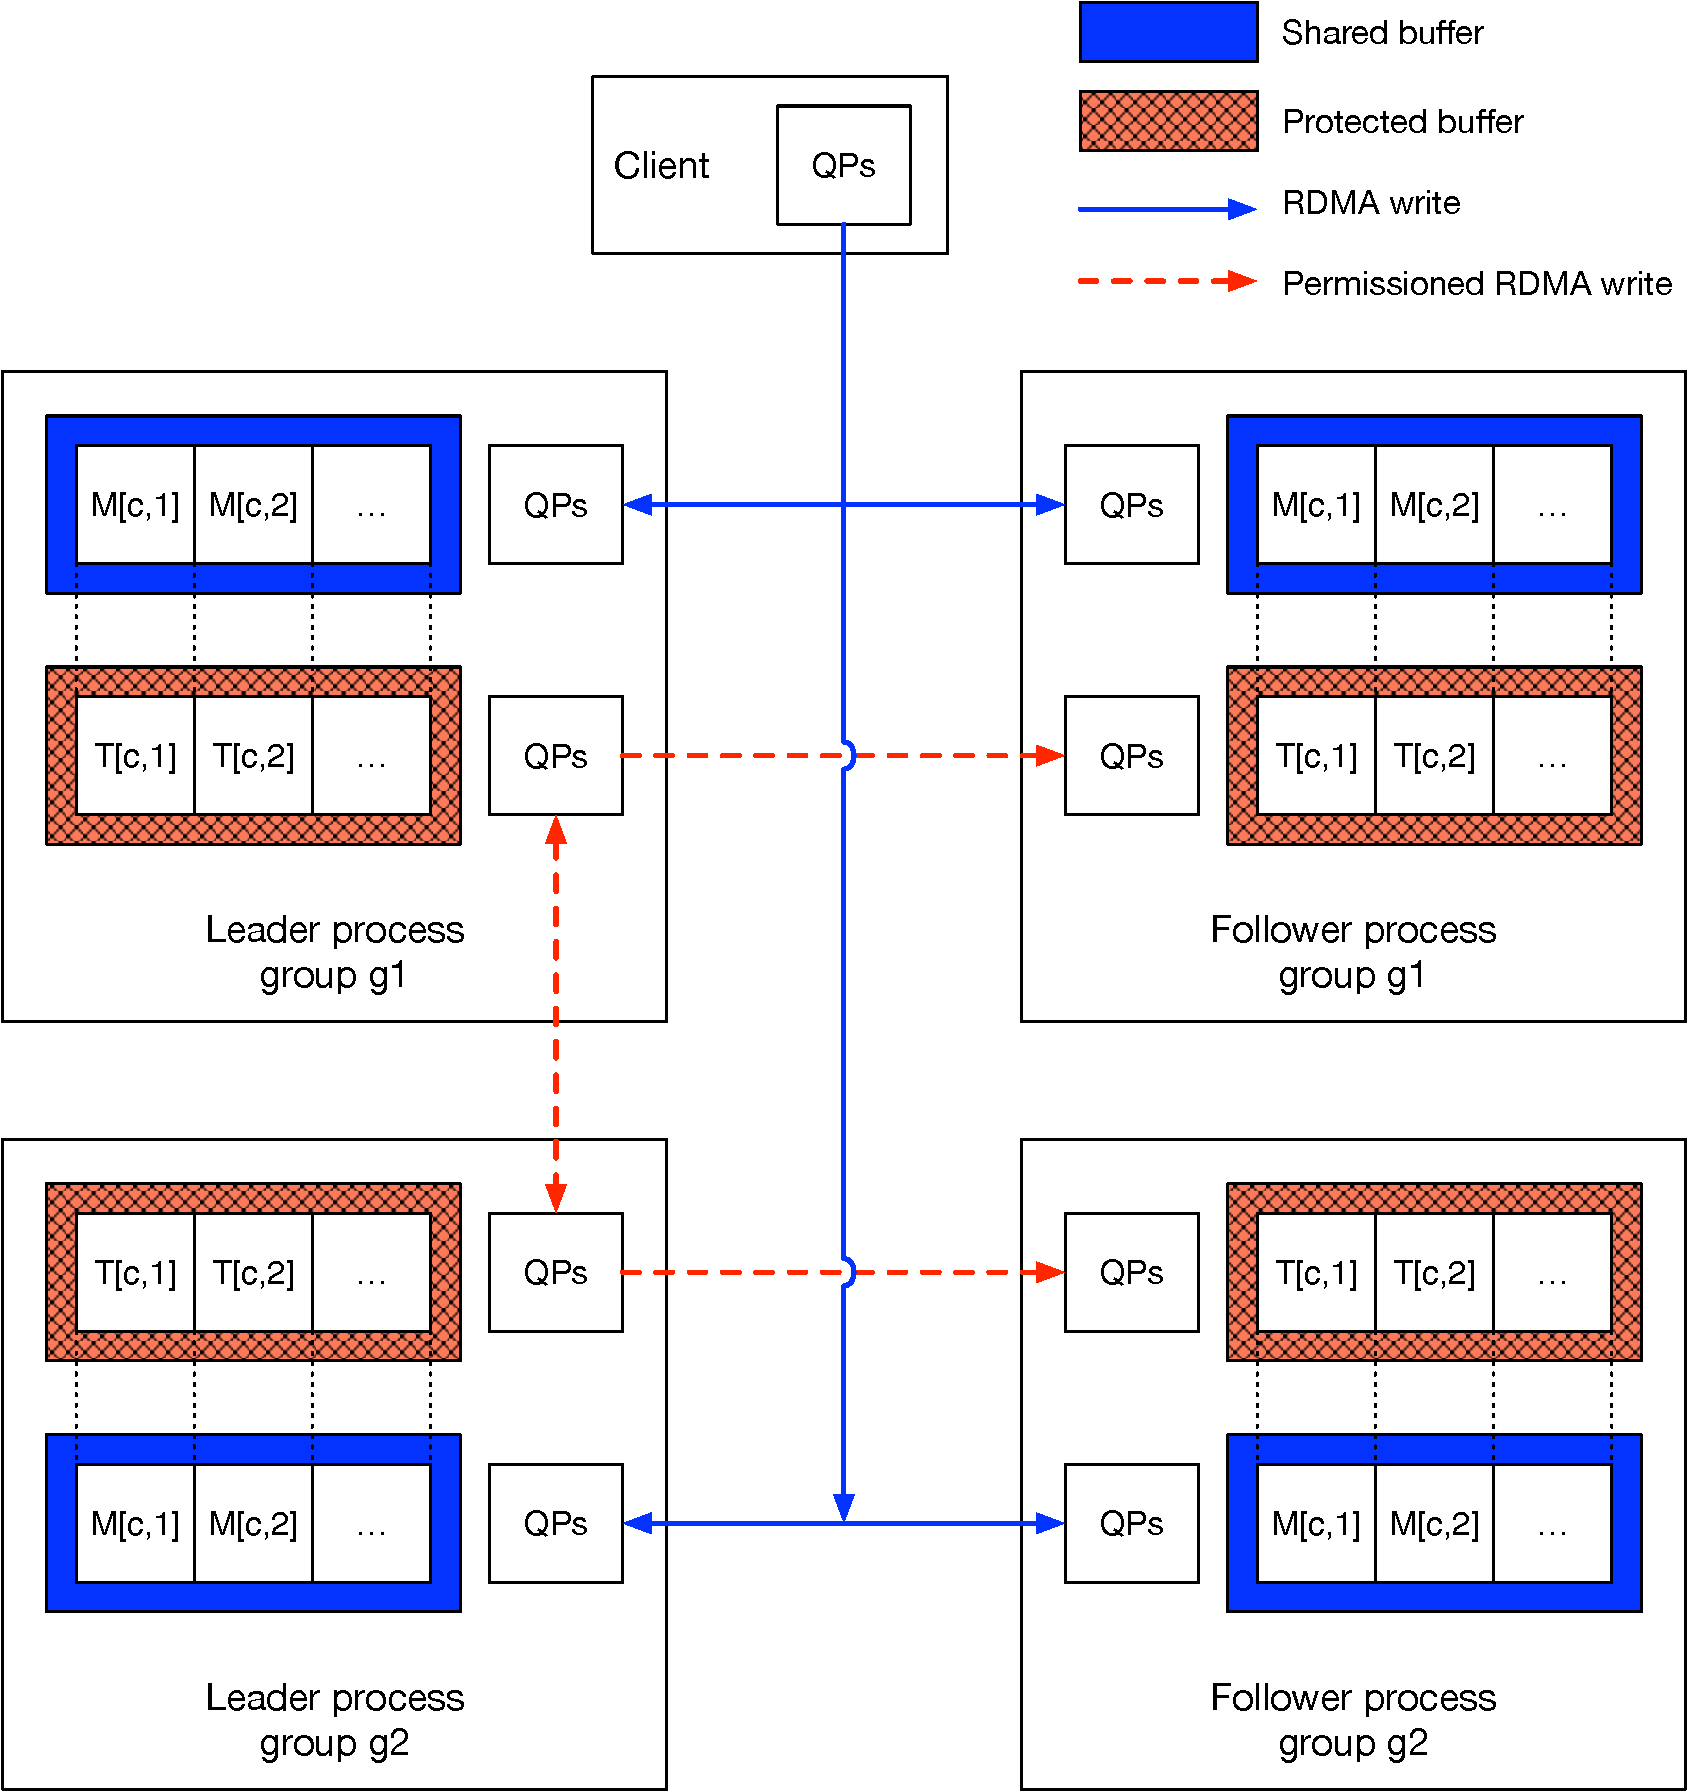
\includegraphics[width=1\linewidth]{figures/architecture2}
  \caption{\libname's memory layout. The normal execution proceeds in three steps: in step 1, the client writes a multicast message in the memory of all destination processes; in step 2 the leader of each destination group proposes and writes a timestamp for the message in the memory of its followers and other leaders; in step 3 the leaders propagate the timestamp written by other leaders, and the followers acknowledge the proposed timestamps. The message is delivered after step 3.}
%Processes have shared and exclusive memory that can be accessed by RDMA primitives. Exclusive memory access needs permission. A client proposes new message by writing to the shared memory of all processes. Leader processes writes their proposed timestamps to exclusive memory. Follower processes write their acknowledgement to the shared memory}
  \label{fig:arch}
\end{figure}


\libname consists of the following main components:
\begin{itemize}
  \item \emph{Memory management.} This component handles the shared buffer and the protected buffer (detailed in \S\ref{sec:ds-structs}). While all processes have read and write access to the shared buffer of a process, only the leader of each group has write permission to the protected buffer of a process. 
  %Each process grants and revokes write permission to its protected buffer, to ensure only one leader of each group has write access at a time.
  \item \emph{RDMA communication.} This component provides functions to read and write remote memory, used by the normal execution component, and to send and receive messages, used by the failure handling module.
  \item \emph{Normal execution.} The normal protocol execution (detailed in \S\ref{sec:normalcase}) is invoked when there is a sole leader per group with support of at least a majority of processes in its group. A leader is responsible for proposing the group's timestamp for a new multicast message, and propagating timestamps from other groups to followers of its own group.
  \item \emph{Failure handling.} Upon detecting the failure of a leader, processes in a group elect a new leader. The new leader must ensure that its execution is consistent with the execution of the previous leader (detailed in \S\ref{sec:failurecase}).
  \item \emph{Leader election.} \libname requires processes to detect a slow or crashed leader, and elect a new leader. Leader election is not assumed to be perfect: the protocol ensures safety despite multiple leaders in a group. To ensure progress, though, eventually every group should elect a single operational and stable leader \cite{Aguilera2019,L98}.
Stable leader election can be implemented in the partially synchronous model \cite{Aguilera2001}.
\end{itemize}

\subsection{Data structures}
\label{sec:ds-structs}

Algorithm~\ref{alg:data_struct} presents the data structures used by processes in \libname.
Every server process has a shared buffer $M$ per client $c$, where slot $M[c,i]$ contains the $i$-th message $msg$ multicast by client $c$, the groups $dst$ the message is addressed to, and an address vector $ptr$, where $ptr[g,p]=j$ means that at process $p$ in group $g$ message $msg$ is stored in slot $M[c,j]$. 
The address vector is used by a process to know where to write in the memory of another process addressed by the message.
Servers compute the message's timestamp $tmp$, based on the timestamps proposed by the leader of each destination group, and the acknowledgements from the members of the leader's group, stored in vector $ack$.
%A timestamp is a tuple $(cnt,pid)$, where $cnt$ is a scalar and $pid$ is a process identifier, used to break ties.
A multicast message state $stat$ can be null ($\perp$), pending a final timestamp (\mcast), assigned a final timestamp (\ordered) or delivered (\done).

To compute a message's timestamp, each server process has a protected buffer $T$, where the $i$-th slot $T[c,i]$ matches the corresponding slot $M[c,i]$ in the shared buffer $M$ associated with $c$.
The slot contains a timestamp vector $tmp$ and a round vector $rnd$, each one with an entry per group $g$: $tmp[g]$ contains the timestamp proposed by the current leader in $g$ in round $rnd[g]$.
Timestamps and rounds are tuples $\langle cnt,pid \rangle$, where $cnt$ is a scalar and $pid$ is a process identifier. 
It follows that $\langle cnt,pid \rangle > \langle cnt',pid' \rangle$ iff $cnt > cnt'$, or $cnt = cnt'$ and $pid > pid'$.
We further assume that $time(\langle cnt,pid \rangle)=cnt$.

To multicast a message, a client writes the message in the shared buffer of each process in the groups addressed by the message.
To know in which entry the multicast message must be written, the client keeps an address vector $ptr$ with an entry per group and per process in the group.

Process $p$'s local state includes a $clock$, used to compute logical timestamps, $p$'s current round, used when $p$ is the leader of the group, vector $Leader$ with $p$'s view on the current leader of each group, and vector $Round$, where entry $Round[g]$ contains the largest round $p$ has accepted from $Leader[g]$.


\begin{algorithm}
\footnotesize

\begin{distribalgo}[1]

\STATE{Each server has a shared buffer $M$ and a protected buffer $T$ per client $c$;
each slot in $M$ stores a multicast message; the corresponding slot in $T$ stores the message's timestamps}	
\vspace{1.0mm}
\INDENT{Each slot $M[c,i]$ contains the following information:}
	\STATE $msg$: the message $m$ multicast by client $c$
	\STATE $dst$: destination groups $m$ is addressed to
	\STATE $ptr[1..k,1..n]$: for each $g$ in destination, slot with $msg$ at processes in $g$; $null$ if $g$ is not in the message's destination
	\STATE $tmp$: the timestamp of $m$, initially $\langle 0,0 \rangle$
	\STATE $ack[1..k,1..n]$: for each $g$ in destination, acknowledgment of timestamp in $T[c,i].tmp[g]$ from processes in $g$
	\STATE $stat$: state of $m$: $\perp$ (initially), \mcast, \ordered\ or \done
\ENDINDENT
\vspace{1.0mm}
\INDENT{Each entry $T[c,i]$ contains the following information:}
	\STATE $tmp[1..k]$: timestamp proposed by leader of group $g$
	\STATE $rnd[1..k]$: the round of $g$'s leader, initially $\langle 0,0 \rangle$
\ENDINDENT
\vspace{1.0mm}
\STATE{Each client $c$ has vector $ptr[1..k,1..n]$, with the next available slot in buffers $M$ and $T$ per group $g$ and process $p$}
\vspace{1.0mm}

\INDENT{Each server $p$ at group $g$ also has:}
	\STATE $clock$: logical timestamp counter at $p$, initially $\langle 0,p \rangle$
	\STATE $round$: the round of $p$, when leader, initially $\langle 0,p \rangle$
	\STATE $Leader[1..k]$: the leader at each group
	\STATE $Round[1..k]$: last accepted round at each group
\ENDINDENT

\vspace{2.0mm}

%\INDENT{\textbf{procedure} $Relay(c,msg,dst,ptr)$}
%	\INDENT{for each $h$ in $dst$: for each $q$ in $h$}
%		\STATE \rdwrite{q}{M[c,ptr[q]].msg}{msg}
%		\STATE \rdwrite{q}{M[c,ptr[q]].dst}{dst}
%		\STATE \rdwrite{q}{M[c,ptr[q]].ptr}{ptr}
%		\STATE \rdwrite{q}{M[c,ptr[q]].stat}{\mcast}
%	\ENDINDENT
%\ENDINDENT
%\vspace{2.0mm}
%\INDENT{\textbf{function} $increment((cnt,pid))$}
%	\STATE $cnt \leftarrow cnt + 1$
%	\STATE return $(cnt,pid)$
%\ENDINDENT
%\vspace{2.0mm}
%
%\vspace{2.0mm}
%\INDENT{\textbf{function} $max((cnt_1,pid_1),(cnt_2,pid_2))$}
%	\IF{$cnt_1 > cnt_2$ \textbf{or} $(cnt_1=cnt_2\ \band\ pid_1 > pid_2)$}
%		\STATE return $(cnt_1,pid_1)$
%	\ELSE
%		\STATE return $(cnt_2,pid_2)$
%	\ENDIF
%\ENDINDENT
%\vspace{2.0mm}


\caption{Data structures}
\label{alg:data_struct}
\end{distribalgo}
\end{algorithm}




%\begin{figure}[ht!]
%  \centering
%  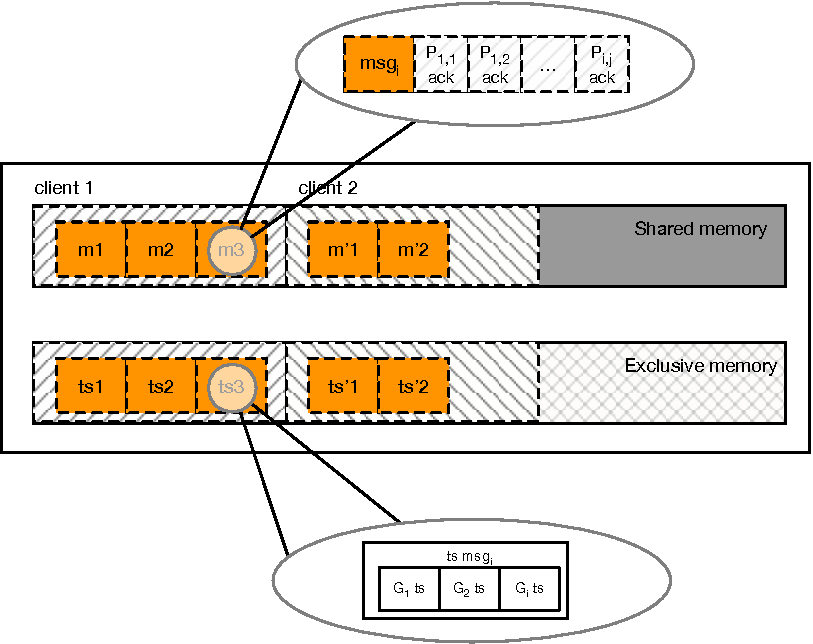
\includegraphics[width=1\linewidth]{figures/memory}
%  \caption{Memory layout of \libname. Each process has shared and exclusive memory
%  space. All other processes can access shared memory. Only leader can access
%  exclusive memory }
%  \label{fig:normal_operation_time}
%\end{figure}







\subsection{Normal execution}
\label{sec:normalcase}

\libname is optimized for the normal case, when a message is addressed to groups whose leaders are operational and stable.
Algorithm \ref{alg:normal_case} presents \libname's normal execution, and 
Figure~\ref{fig:normal_operation_time} illustrates one normal execution.
We explain next the behavior of each one of the tasks in Algorithm \ref{alg:normal_case}.

\begin{itemize}
\item \emph{Task 1.} To multicast message $m$, client $c$ first calculates the next available slot in the buffer of every process addressed by $m$. Then, $c$ invokes the $Relay$ procedure, which copies the message, its destination, and the address vector for $m$ in the message buffer of every process addressed by $m$.

\begin{figure}[ht!]
  \centering
  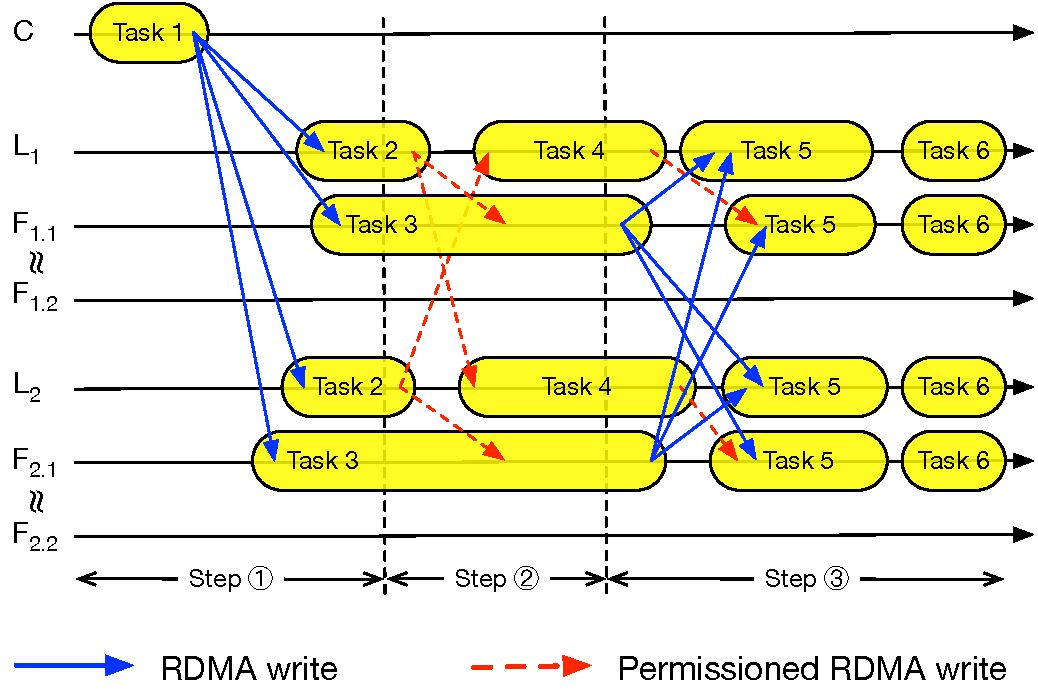
\includegraphics[width=1\linewidth]{figures/execution}
  \caption{Normal execution of \libname. We show the steps at one follower per group only to avoid cluttering.}
  \label{fig:normal_operation_time}
\end{figure}

\item \emph{Task 2.} Once leader process $L$ in group $g$ reads $m$ from its message buffer, it computes a
group-wise timestamp for $m$ and writes the proposed timestamp 
in the protected timestamp buffer of all follower processes in the leader's group $g$, and all leader processes 
of other groups in the destination of $m$.
If a remote write is denied, then $L$ ends the task since another process in $g$ became leader.

\item \emph{Task 3.} When a follower detects that a multicast message has been assigned a timestamp by the group leader, it updates its clock.
This is done to ensure that timestamps from a group are monotonically increasing (necessary in case the process becomes leader).
Then, the follower acknowledges that it has read this timestamp by writing the round used by the leader in its entry in the $ack$ vector of every process in the destination of the message.
The follower detects the leader proposed timestamp by checking whether the round of the timestamp matches the round associated with the  leader. 
This assumes that both the timestamp and the round have been updated by the leader.
We discuss in Section~\ref{sec:implementation} how we ensure this with RDMA.

\item \emph{Task 4.} 
When the leader $L$ in $g$ reads a timestamp written by a leader in another group, $L$ updates its local clock with the timestamp, to ensure that any future proposed timestmaps will be bigger, and writes the read timestamp in the memory of each one of its followers.
This task is executed by the leader of a group only, since only the leader is updated with timestamps from the leader of another group (see Task 2).
The reason why only the leader of a group is updated is to ensure that any timestamps assigned by the leader are consistent with any other timestamps assigned by the group.
%, similarly to other leader-follower-based protocols \cite{gotsman2019white, Junqueira2011}.
%Once each involved process $P$ belongs to $m.dst$ \lread message $m$ in its
%local buffer, $P$ mark the message as pending, and starts polling from it
%exclusive memory for timestamps of $m$ (Task 4 algorithm~\ref{alg:normal_case}).

\item \emph{Task 5.} 
When a message has a timestamp proposed by a leader from each destination group of the message, and a quorum of processes in each destination group agrees with the proposed timestamp, the message becomes ordered.

\item \emph{Task 6.} 
A process delivers an ordered message when it can assert that no other messages can be assigned a smaller timestamp.

\end{itemize}

In the normal case, a message multicast by a client to multiple groups is delivered by the leaders and the followers of the addressed groups after three RDMA write delays (see Figure~\ref{fig:normal_operation_time}).
In Section~\ref{sec:extensions}, we discuss how messages addressed to a single group can be delivered by the group's leader after two RDMA write delays.

%!TEX root =  main.tex

\newcommand{\rdwrite}[3]{WRITE\ensuremath{(@#1\!\rightarrow\!#2, #3)}}	% rdwrite(addr,val) 
%\newcommand{\rmm}[2]{\ensuremath{@#1\!\rightarrow\!#2}}
\newcommand{\band}{\textbf{and}}
\newcommand{\mcast}{\textsf{mcast}}
\newcommand{\ack}{\textsf{ack}}
\newcommand{\ordered}{\textsf{ordered}}
\newcommand{\done}{\textsf{done}}
\newcommand{\myack}{\textsf{ack}}

\begin{algorithm}
\footnotesize

\begin{distribalgo}[1]

\STATE{Each server has a shared buffer $M$ with multicast messages and a protected buffer $T$ with message timestamps per client $c$}	
\vspace{1.0mm}
\INDENT{Each entry $M[c,i]$ contains the following information:}
	\STATE $msg$: the message $m$ multicast by client $c$
	\STATE $tmp$: the timestamp of $m$, computed by the algorithm
	\STATE $dst$: destination groups $m$ is addressed to
	\STATE $slot[]$: buffer entry with message at each process
	\STATE $ack[p]$: acknowledgement of timestamp in $tmp[p]$
	\STATE $stat$: state of message $m$: \mcast, \ordered\ or \done
\ENDINDENT
\vspace{1.0mm}
\INDENT{Each entry $T[c,i]$ contains the following information:}
	\STATE $tmp[g]$: timestamp proposed by group $g$
	\STATE $rnd[g]$: round in which $g$'s leader proposed timestamp
\ENDINDENT
\vspace{1.0mm}
\STATE{Each client has structure $next[p]$ containing the next entry in the buffer at $p$}
\vspace{1.0mm}

\INDENT{Each server $p$ at group $g$ also has:}
	\STATE{$Leader[g]$ the identifier of the leader at $g$ (as seen by $p$)}
%	\INDENT{$round$: $p$'s current round in any execution}
%		\STATE{incremented when becomes leader}
%		\STATE{unique per process}
%	\ENDINDENT
	\STATE{$clock$: logical timestamp counter at process $p$}
\ENDINDENT
\vspace{1.0mm}
\caption{Data structures}
\label{alg:data_struct}
\end{distribalgo}
\end{algorithm}

\begin{algorithm}
\footnotesize

\begin{distribalgo}[1]

\STATE{Client $c$ multicasts message $m$ to groups in $dst$ as follows:}
\vspace{1.0mm}
	\STATE for each $h$ in $dst$: for each $q$ in $h$: increment $next[q]$
	\INDENT{for each $h$ in $dst$: for each $q$ in $h$}
		\STATE \rdwrite{q}{M[c,next[q]].msg}{m}
		\STATE \rdwrite{q}{M[c,next[q]].dst}{dst}
		\STATE \rdwrite{q}{M[c,next[q]].slot}{next}
		\STATE \rdwrite{q}{M[c,next[q]].tmp}{0}
		\STATE \rdwrite{q}{M[c,next[q]].stat}{\mcast}
	\ENDINDENT
\vspace{1.0mm}

\STATE Server $p$ in group $g$ executes as follows:
\vspace{1.0mm}
\WHEN[\textbf{Task 1}]{$\exists c,i:\!M[c,i].stat\!=\!\mcast$\ \band\ 
		$p\!=\!Leader[g]$\hspace{-2mm}}
	\STATE increment $clock$
	\INDENT{for each follower $q$ in $g$ \band\ each leader $q$ in $M[c,i].dst$}
		\STATE $j \leftarrow M[c,i].slot[q]$
		\STATE \rdwrite{q}{T[c,j].tmp[g]}{clock}
		\IF{write denied}
			\STATE request permission (Phase 1)
			\STATE end task
		\ENDIF
	\ENDINDENT	
\ENDWHEN
\vspace{1.0mm}

\WHEN[\textbf{Task 2}]{$\exists c, i\!:\!M[c,i].stat\!=\!\mcast$\ \band \\
		\hspace{14mm} $T[c,i].tmp[g]\!\neq\!0$\hspace{-2mm}}
	\STATE update $clock$ with $T[c,i].tmp[g]$
	\INDENT{for each $h$ in $M[c,i].dst$: for each $q$ in $h$}
		\STATE $j \leftarrow M[c,i].slot[q]$
		\STATE \rdwrite{q}{M[c,j].ack[p]}{\myack}
	\ENDINDENT	
\ENDWHEN
\vspace{1.0mm}

\WHEN[\textbf{Task 3}]{$\exists c, i, h\!:\!M[c,i].stat =$ \mcast\ \band \\
		\hspace{14mm} $T[c,i].tmp[h] \neq 0$ \band\ $h \neq g$ \hspace{-2mm}}
	\STATE update $clock$ with $T[c,i].tmp[g]$
	\INDENT{for each follower $q$ in $g$}
		\STATE{$j \leftarrow M[c,i].slot[q]$}
		\STATE \rdwrite{q}{T[c,j].tmp[h]}{T[c,i].tmp[h]}
		\INDENT{if write denied then}
			\STATE{request permission (Phase 1)}
			\STATE end task
		\ENDINDENT
	\ENDINDENT	
\ENDWHEN
\vspace{1.0mm}

\WHEN[\textbf{Task 4}]{$\exists c, i, h\!:\!M[c,i].stat =$ \mcast\ \band\ $\exists\!$ quorum $Q$ in $h$: \\
	\hspace{5mm} for each $q$ in $Q$: $M[c,i].ack[q] = \ack$}
			\STATE $M[c,i].tmp \leftarrow$ \\
				\hspace{10mm} $max\{ M[c,i].tmp, M[c,i].tmp[Leader[h]] \}$
			\IF{for each group $h$ in $M[c,i].dst$: $\exists\!$ quorum $Q$ in $h$: \\
	\hfill for each $q$ in $Q$: $M[c,i].ack[q] = \ack$}
						\STATE $M[c,i].stat \leftarrow$ \ordered
			\ENDIF
%			\STATE{include $(m,t_{final})$ in $ordered$}
%			\STATE{remove $(m,-,-)$ from $pending$}		
\ENDWHEN
\vspace{1.0mm}


\WHEN[\textbf{Task 5}]{$\exists c, i\!:\!M[c,i].stat =$ \ordered\ \band \\
	\hspace{10mm} $\nexists d,j\!:\!M[d,j].stat \in \{ \ordered, \mcast \}$ \band\ \\
	\hspace{10mm} $M[d,j].tmp < M[c,i].tmp$}
		\STATE{deliver $m$}
		\STATE $M[c,i].stat \leftarrow$ \done
\ENDWHEN
\vspace{1.0mm}

\caption{Algorithm}
\label{alg:normal_case}
\end{distribalgo}
\end{algorithm}

% %!TEX root =  main.tex
\begin{algorithm*}
\footnotesize

\begin{distribalgo}[1]

\INIT
	\STATE $ts \leftarrow 0$
	\COMMENT{P's logical clock}
	\STATE $pending \leftarrow \emptyset$
	\COMMENT{set of message to be ordered}
	\STATE $ordered \leftarrow \emptyset$
	\COMMENT{set of message already ordered, to be delivered}
	\STATE $pending_{ts} \leftarrow \emptyset$
	\COMMENT{set of pending slots for timestamps}
	% \STATE $pending_{ack} \leftarrow \emptyset$
	% \COMMENT{set of pending slots for acknowledgements}
	\STATE $bal \leftarrow 0$
	\COMMENT{ballot number}
	\STATE $seq \leftarrow 0$
	\COMMENT{sequence number}
	\STATE $curSeq \leftarrow 0$
	\COMMENT{P's current sequence number}
	\STATE $\buffer \leftarrow NULL$
	\COMMENT{P's local buffer}
	\vspace{2.0mm}
\ENDINIT
\vspace{2.0mm}

\INDENT{\colorbox{\coloralgo}{to a-mcast message m	:}}
	\FORALL[\textbf{Task 1}] {$p \in G \mid \forall G \in  m.dest$}
		\TRIGGER {$ \langle rdma, \WRITE \mid p, [m] \rangle$}
		\COMMENT{remote-write m to memory of all processes belong to all involved groups}
	\ENDFOR
\ENDINDENT
\vspace{2.0mm}

\INDENT{\colorbox{\coloralgo}{leader process $P_L$ of group $G$}}
	\UPON[\textbf{Task 2} on receive message $m$ in local buffer]{$\langle \buffer, \READ \mid m \rangle$}
		\STATE $dest \leftarrow \{\forall p \mid p \in G\} \cup \{\forall p \in G_i \mid G_i \in m.dest \wedge p.isLeader\}$
		\COMMENT{set of all processes in G and all leaders of involved groups}
		\STATE $ts \leftarrow ts + 1$
		\COMMENT{increase local timestamp}
		\STATE $seq \leftarrow seq + 1$
		\COMMENT{increase sequence number}
		\FORALL {$p \in dest$}
			\TRIGGER {$ \langle rdma, \WRITE \mid p, [P_L, bal, seq, ts] \rangle$}
			\COMMENT{remote-write $P_l$'s timestamp with ballot $bal$ and sequence $seq$ to all process $\in dest$ set}
		\ENDFOR
	\ENDUPON
	\vspace{2.0mm}

	\UPON[\textbf{Task 3} on receive timestamp $ts_l$ of a leader $P_l$ in local buffer]{$\langle \buffer, \READ \mid [P_l, bal_l, seq_l, ts_l] \rangle$}
		\STATE $seq \leftarrow seq + 1$
		\COMMENT{increase sequence number}
		\FORALL {$p \in G$}
			\TRIGGER {$ \langle rdma, \WRITE \mid p, [P_l, bal, seq, ts_l] \rangle$}
			\COMMENT{propagate $P_l$'s timestamp $ts_l$ with its ballot and sequence number $seq$ to all process $\in dest$ set}
		\ENDFOR
		\STATE $ts \leftarrow max(ts, ts_l)$
	\ENDUPON
\ENDINDENT
\vspace{2.0mm}

\INDENT{\colorbox{\coloralgo}{any process $P$ of group $G$}}
	\UPON[\textbf{Task 4} on receive message $m$ in local buffer]{$\langle \buffer, \READ \mid m \rangle$}
		% \STATE do $\READ(ts, L)$
		\STATE $pending \leftarrow pending \cup \{m\}$
		\COMMENT{include m in pending messages set}
		% \COMMENT{polling timestamp of leader of its own group}
		\STATE $pending_{ts} \leftarrow pending_{ts} \cup \{\langle m_{id}, G \rangle \mid \forall G, G \in m.dest \}$
	\ENDUPON
	\vspace{2.0mm}

	\WHEN{true}
		\IF[\textbf{Task 5} ]{$ \exists \langle m_{id}, G \rangle \in pending_{ts} : ts_G \neq 0 $}
			\STATE $ts \leftarrow max(ts, ts_G)$
            		\COMMENT{Lamport’s rule to update logical clocks}
            		\FORALL {$p \in m.dest$}
            			\TRIGGER {$ \langle rdma, \WRITE \mid p, [P, ack] \rangle$}
            			\COMMENT{remote-write P's ack to memory of all involved processes}
            		\ENDFOR

			% \STATE $pending_{ack} \leftarrow pending_{ack}$ \textbackslash $\{ \langle m_{id}, G \rangle \}$
            		\STATE $pending_{ts} \leftarrow pending_{ts} \cup \{ \langle m_{id}, G, c_w \rangle \}$
            		\COMMENT{include $\langle ts_l, c_w, m \rangle$ in pending timestamps set}

			\WHILE[refer to note]{$\exists \langle m_{id}, G, c_w \rangle \in pending_{ts} : c_w = curSeq + 1$}
            			\STATE $pending_{ts} \leftarrow pending_{ts}$ \textbackslash $\{\langle m_{id}, G \rangle\}$
            			\COMMENT{remove $\langle m_{id}, G \rangle$ from ts pending set}
            			\STATE  $curSeq = curSeq + 1$
            			\COMMENT{increase current sequence number}
            		\ENDWHILE

            		\WHILE[]{$\exists m \in pending : isFulfilled(m) = true$}
            			\STATE $t \leftarrow max(ts_i)$
            			\COMMENT{$t$ is the largest timestamp between all timestamps $ts_i$ populated by all leaders}
            			\STATE $pending \leftarrow pending$ \textbackslash $\{m\}$
            			\COMMENT{remove $m$ from pending set}
            			\STATE $ordered \leftarrow ordered \cup \langle m, t \rangle$
            			\COMMENT{include $\langle m, t \rangle$ in ordered set}
            		\ENDWHILE

            		% \WHILE {$\exists \langle m,t \rangle \in ordered : t < min(\forall t_i \in pending) \wedge \newline
            		% 		\hspace*{11.7em} t < min(\forall t_i \in ordered)$:}
            		\WHILE {$\exists \langle m,t \rangle \in ordered : t < min(\forall t_i \in pending) \wedge t < min(\forall t_i \in ordered)$:}
            			\STATE $ordered \leftarrow ordered$ \textbackslash $\{m\}$
            			\STATE deliver $m$
            		\ENDWHILE
		\ENDIF
	\ENDWHEN
\ENDINDENT
\vspace{4.0mm}

% \INDENT{\colorbox{\coloralgo}{\textbf{function} \rwrite$(dest, data\dots)$}}
% 	\STATE rdma-write $[data\dots]$ to $dest$'s shared buffer
% \ENDINDENT
% \vspace{2.0mm}

% \INDENT{\colorbox{\coloralgo}{\textbf{function} \READ$(data\dots)$}}
% \STATE atomic-read $[data\dots]$ from local buffer
% \ENDINDENT
% \vspace{2.0mm}

\INDENT{\colorbox{\coloralgo}{\textbf{function} isFulfilled$(m)$}}
	\IF[m receives ts of all involved groups and acks from majority processes]{$\forall G \mid G \in m.dst \wedge \newline
	\hspace*{3.5em} ts_G \neq 0 \wedge \newline
	\hspace*{3.5em} \langle m_{id}, G, c_w \rangle \notin pending_{ts} \wedge \newline
	\hspace*{3.5em} $ received acks for $ts_G$ from majority:}
		\RETURN true
	\ELSE
		\RETURN false
	\ENDIF
\ENDINDENT

\caption{Normal case execution}
\label{alg:normal_case}
\end{distribalgo}
\end{algorithm*}


\subsection{Handling failures}
\label{sec:failurecase}

%%!TEX root =  main.tex
\begin{algorithm*}
  \footnotesize
  
  \begin{distribalgo}[1]
  
  \INIT
    \STATE $\Pi \leftarrow \{p_1, p_2, ..., p_n\}$
    \COMMENT{Set of all processes in the system}    
    \STATE $\Gamma \leftarrow \{G_1, G_2, ..., G_n\}$
    \COMMENT{Set of process groups in the system}    
    \STATE $\beta \leftarrow \emptyset$
    \COMMENT{Map of ballot numbers stored for each group}
    \STATE $\Delta \leftarrow \emptyset$
    \COMMENT{Map of leader process of each group}
    \STATE $M \leftarrow \emptyset$
    \COMMENT{Map of messages and their status on each group}
    \vspace{2.0mm}
  \ENDINIT
  \vspace{2.0mm}
  
  \INDENT{\colorbox{\coloralgo}{elected process $P_L$ of group G:}}
    % \FORALL {$M \in \Gamma$}
    %   \STATE $pending[g] \leftarrow \emptyset$
    %   \STATE $ordered[g] \leftarrow \emptyset$
    % \ENDFOR

    \STATE $bal \leftarrow bal + 1$
    \COMMENT{increase ballot number}
    \FORALL[\textbf{Task 6}] {$p \in \Pi$}
      \TRIGGER {$ \langle rdma, \SEND \mid p, [1A, G, P_L, bal] \rangle$}
      \COMMENT{elected process sends 1A message to all processes of all groups}
    \ENDFOR
    \vspace{2.0mm}

    \UPON[\textbf{Task 8} on receive 1B message from process $P$ of group Q]{$\langle \RECV \mid [1B, Q, state] \rangle$}
      \FORALL {$m \in state$}
        \STATE $M[m.id] \leftarrow M[m.id] \cup m$
      \ENDFOR
    \ENDUPON
    \STATE{wait until receive 1B messages from quorum of all group $Q \in \Gamma$}

    \STATE{$sync_{settle} \leftarrow \emptyset$}
    \STATE{$sync_{reacked} \leftarrow \emptyset$}
    \STATE{$sync_{reset} \leftarrow \emptyset$}

    \FORALL {$m_{id} \in M$}      
      \IF{m is fulfilled on some process $P \in m.dest$}
        \STATE{$sync_{settle} \leftarrow sync_{settle} \cup m$}
      \ELSE[m is not fulfilled on any process $P \in m.dest$]
        % \STATE{$sync_{settle} \leftarrow sync_{settle} \cup m$}
        \IF{timestamp of G reaches quorum of acks on some process $P \in m.dest$}
          \STATE{$sync_{reacked} \leftarrow sync_{reacked} \cup m$}
        \ELSE[timestamp of G does not reach quorum of acks on any process $P \in m.dest$]
          \STATE{$sync_{reset} \leftarrow sync_{reset} \cup m$}
        \ENDIF
      \ENDIF 
    \ENDFOR

    \STATE $dest \leftarrow \{\forall p \mid p \in G\} \cup \{\forall p \in G_i \mid p.isLeader\}$
		\COMMENT{set of all processes in G and all leaders}
    \TRIGGER {$ \langle rdma, \SEND \mid p, [SYNC, P_L, sync_{settle}, sync_{acked}] \rangle$}
    \COMMENT{send sync state}

  \ENDINDENT
  \vspace{2.0mm}
  
  \INDENT{\colorbox{\coloralgo}{any process P of group Q:}}
    \UPON[\textbf{Task 7} on receive 1A message from process $P_L$ of group G with ballot number $bal$]{$\langle \RECV \mid [1A, G, P_L, bal] \rangle$}
      \IF[if the ballot number is greater than stored ballot number of G]{$ bal > \beta[G]$}
        \STATE{$\beta[G] \leftarrow bal$}
        \COMMENT{update the local ballot number for group G}
        \TRIGGER {$ \langle buffer, \REVOKEPERM \mid \Delta[G] \rangle$}
        \COMMENT{revoke permission of the previous leader of group G}
        \STATE{$\Delta[G] \leftarrow P_L$}
        \COMMENT{update the leader of group G}      
        \TRIGGER {$ \langle buffer, \GRANTPERM \mid \Delta[G] \rangle$}
        \COMMENT{revoke permission of the previous leader of group G}
        \STATE{$state \leftarrow \{ m \mid m \in pending \cup order \wedge Q \in m.dest \}$}
        % \STATE{$state_o \leftarrow \{ m \mid m \in ordered \wedge Q \in m.dest \}$}        
        \TRIGGER {$ \langle rdma, \SEND \mid P_L, [1B, Q, state] \rangle$}
        \COMMENT{send back 1B message with the set of pending and ordered messages}
      \ENDIF
    \ENDUPON
    \vspace{2.0mm}

    \UPON[\textbf{Task 9} on receive SYNC message]{$\langle \RECV \mid [SYNC, P_L, sync_{settle}, sync_{reacked}, sync_{reset}] \rangle$}
      \FORALL {$m \in sync_{settle}$}
        \STATE{copy m state to local buffer}
        \STATE{$ordered \leftarrow ordered \cup m$}
        \COMMENT{update local state of m and add m to the queue to be delivered}
      \ENDFOR
      \FORALL {$m \in sync_{reacked}$}
        \STATE{copy m state to local buffer}
        \IF{P is Leader}
          \STATE{perform \textbf{Task 3}}
          \COMMENT{re-propagate m's timestamp}
        \ELSE
          \STATE{perform \textbf{Task 5}}
          \COMMENT{re-ack for m's timestamp}
        \ENDIF
      \ENDFOR
      \FORALL {$m \in sync_{reset}$}
        \IF{P is $P_L$}
          \STATE{perform \textbf{Task 2}}
          \COMMENT{rerun whole process for m}
        \ENDIF
      \ENDFOR
    \ENDUPON
   
  \ENDINDENT
  \vspace{2.0mm}
  
  
  \caption{Leader election and recovery}
  \label{alg:normal_case}
  \end{distribalgo}
  \end{algorithm*}
  

When a process becomes leader, it needs to catch up with the previous leader.
In the following, we describe how the newly elected leader does this.
The procedure uses both shared memory and message passing for communication.
In RDMA, message passing is less efficient than shared memory, but it reduces complexity, as we do not have to handle concurrent accesses to shared memory.
Since failures are hopefully rare, we consider that trading performance for simplicity is acceptable.

\begin{itemize}
\item \emph{Task 7.} 
When a process that will become the next leader of the group suspects the current leader, it determines its \emph{first undecided slot (FUS)} per client in its shared buffers.
A slot is undecided if its state is equal to \mcast. 
Then, the new leader chooses a round and sends a catch-up message to every server process in the system.
Since slot $i$ in the new leader's buffer may correspond to a different slot at another process, the new leader must convert its FUS into one that is meaningful for the contacted process.

\item \emph{Task 8.} 
A process $p$ will consider a catch-up message from new leader $q$ in group $h$ if $q$ has picked a round bigger than the current round for $h$ at $p$.
This is a requirement from Paxos, to ensure that a new leader will not decide on a value different than a previously decided value.
If the catch-up message can be considered, then $p$ grants permission to the shared buffer $T$ to $q$, collects all information requested by $q$, and sends it to $q$.
Finally, $p$ updates $h$'s round and leader.

\item \emph{Task 9.}
When the new leader receives responses for a catch-up request from a quorum of processes in a group, it handles each entry $i$ for every client $c$ received as follows.
First, the process selects the response with the largest round. 
From Paxos, this ensures that if a timestamp has been chosen, it can only be the one with the largest round.
The next steps depend on whether the process received the responses from its own group or not.
If the process received the responses from its own group, then it picks the timestamp in the selected response, if any, or picks a timestamp using its own clock. 
In either case, the process proposes the picked timestamp to all other members of its group and the leaders of the other involved groups.
If the process received the responses from another group, then it forwards the timestamp in the selected response to the followers in its group.
\end{itemize}

We also consider the case of faulty clients, who may fail to update all destinations of a multicast message.

\begin{itemize}
\item \emph{Task 10.} 
When a process detects the failure of a client, it relays all the messages multicast by the faulty client that have not been ordered yet.
This means that only messages in the \mcast\ state need to be relayed.
\end{itemize}

%Firstly, the new leader must choose a new ballot number that is higher than all
%ballot numbers before for its group. A process only reply to the message or
%timestamp that has a ballot number higher than its current value. The new ballot
%number will be included in each timestamp $ts$ of this leader later.
%
%The new leader needs to get the access to the exclusive memory space on (1) the
%followers of its local group, and (2) the leaders of other groups. In order to
%act as a leader, a node must get the write permission from majority of other
%processes in its group. In addition, to tolerate failure of the leaders of other
%groups, the new leader also need to get the write permission from majority of
%processes of other groups. The new leader request the access by issuing a RDMA
%Send (\lle{this could be a \rwrite}) 1A message that includes a new ballot
%number all involved processes. Upon receiving such message, a process first
%checks if the proposed ballot number is higher than the current ballot number it
%stored. In such case, the process revokes access of the old leader, and replies
%to the new leader with an 1B message that also contains the status of all
%message it is processing (i.e., messages that are pending and messages that has
%been fulfilled and are waiting to be delivered)
%
%Once the new leader receives 1B reply from majority processes of each group, it
%must ensure all remote logs are up-to-date with its own. If a message m is
%fulfilled in some processes, the leader stores it in a settled list. If a
%message is not fulfilled in any process, there are two cases: i)  the message
%does not have the timestamp or enough acknowledgements from quorum of processes
%of the group that has failed leader on any process ii) it does have such data on
%some processes.\lle{sloppy sentence}

%!TEX root =  main.tex
\begin{algorithm}
\footnotesize

\begin{distribalgo}[1]

\WHEN[\textbf{Task 7}]{suspect $Leader[g]$ \band\ $p$ is $g$'s next leader}	
%\WHEN[\textbf{Task 7}]{suspect $Leader[g]$ \band\ $p$ is $g$'s next leader}	
	\FOR{each $c$}
		\STATE $\mathit{FUE}[c] \leftarrow i$, where $M[c,i]$ is the first undecided entry %($M[c,i] = \mcast)$
	\ENDFOR
	\STATE $round \leftarrow \langle time(round)+1,g \rangle$
	\INDENT{\textbf{for} each $h$ in $\Gamma$}
		\INDENT{\textbf{for} each $q$}
			\STATE \textbf{for} each $c$: $\mathit{xFUE}[c] \leftarrow M[c,\mathit{FUE}[c]].ptr[h,q]$
			\STATE \textsf{send} $(\textsc{catch\_up}, \mathit{xFUE}, round)$ to $q$
		\ENDINDENT
	\ENDINDENT
\ENDWHEN

\vspace{2.0mm}
\WHEN[\textbf{Task 8}]{\textsf{receive} $(\textsc{catch\_up}, \mathit{FUE}, round)$ from $q$ in $h$ \band\ \\
			\hspace{38mm} $round > Round[h]$}	
		\STATE{grant permission to $q$}
		\STATE $pend \leftarrow \emptyset$
		\FOR{each $c$}
			\STATE let $j$ be the last entry in $M$ such that $M[c,j] \neq \perp$
			\FOR{$i$ in $\mathit{FUE}[c]..j$}
				\IF{$h \in M[c,i].dst$}
					\STATE $pend \leftarrow pend \cup (c,i,M[c,i].msg,M[c,i].dst,$ \\ 
						\hfill $M[c,i].ptr,T[c,i].tmp[g],T[c,i].rnd[g])$
				\ENDIF
			\ENDFOR
		\ENDFOR
		\STATE \textsf{send} $(\textsc{my\_state},pend)$ to $q$
		\STATE $Round[h] \leftarrow round$
		\STATE $Leader[h] \leftarrow q$
\ENDWHEN

\vspace{2.0mm}		
\WHEN[\textbf{Task 9}]{\textsf{receive} $(\textsc{my\_state}, pend)$ from quorum $Q$ in $h$,\\
			\hspace{6mm} including $p$'s response if $g=h$}
		\STATE $bag \leftarrow$ union of all received $pend$ from $h$
		\STATE let $maxts$ be the largest timestamp $tmp$ in $bag$
		\STATE $clock \leftarrow max(clock, time(maxts))$
		\INDENT{\textbf{for} each $(c,i,-,-,-,-,-)$ in $bag$}
%		\INDENT{for each $(c,msg,dst,ptr,tmp,rnd)$ in received $pend$}
			\STATE let $(c,i,msg,dst,ptr,tmp,rnd)$ in $bag$ be such that \\
				\hfill $\nexists (c,i,-,-,-,-,rnd')$ in $bag$ \band\ $rnd' > rnd$
%			\STATE \textbf{wait until} $M[c,i].stat = \mcast$
%		\STATE $Relay(c,msg,dst,ptr)$
		\IF{$g=h$}
			\IF{$rnd > 0$}
				\STATE $t \leftarrow tmp$
			\ELSE
				\STATE $clock \leftarrow clock + 1$
				\STATE $t \leftarrow \langle clock,g \rangle$
			\ENDIF
%			\STATE \textbf{else} $t \leftarrow clock$
			\INDENT{\textbf{for} each $q$ in $g$ \band\ each leader $q$ in $dst$}
%				\STATE $j \leftarrow ptr[q]$
				\STATE \rdwrite{q}{T[c,ptr[q]].tmp[g]}{t}
				\STATE \rdwrite{q}{T[c,ptr[q]].rnd[g]}{round}
				\STATE \textbf{if} write denied \textbf{then} end task
			\ENDINDENT	
		\ELSE
			\INDENT{for each $q$ in $g$}
%				\STATE{$j \leftarrow ptr[q]$}
				\STATE \rdwrite{q}{T[c,ptr[q]].tmp[h]}{tmp}
				\STATE \textbf{if} write denied \textbf{then} end task
			\ENDINDENT	
		\ENDIF
		\ENDINDENT
%		\IF{$T[c,i].rnd[g] > 0$}
%			\STATE $t \leftarrow T[c,i].rnd[g]$
%		\ELSE
%			\STATE $t \leftarrow clock$
%		\ENDIF
		
%	\INDENT{for each group $h$}
%		\STATE{wait for a quorum $Q$ of responses $(1B,round,tmp)$ from $h$}
%		\STATE{$(round, tmp) \leftarrow$  the largest round received}
%		\INDENT{if $round=0$}
%			\STATE{propose $p$'s clock}
%		\ENDINDENT
%		\INDENT{else}
%			\STATE{propose $tmp$}
%		\ENDINDENT
%	\STATE{$Leader[g] \leftarrow p$}
\ENDWHEN
\vspace{2.0mm}

\WHEN[\textbf{Task 10}]{suspect client $c$}	
	\INDENT{for each $i$ such that $M[c,i].stat = \mcast$}
		\STATE $Relay(c,M[c,i].msg,M[c,i].dst,M[c,i].ptr)$
%		\INDENT{for each $h$ in $M[c,i].dst$: for each $q$ in $h$}
%			\STATE $j \leftarrow M[c,i].ptr[q]$
%			\STATE \rdwrite{q}{M[c,j].msg}{M[c,i].msg}
%			\STATE \rdwrite{q}{M[c,j].dst}{M[c,i].dst}
%			\STATE \rdwrite{q}{M[c,j].ptr}{M[c,i].ptr}
%%			\STATE \rdwrite{q}{M[c,j].tmp}{0}
%			\STATE \rdwrite{q}{M[c,j].stat}{\mcast}
%		\ENDINDENT
	\ENDINDENT
\ENDWHEN
\vspace{2.0mm}

\caption{Handling failures and suspicions}
\label{alg:failures}
\end{distribalgo}
\end{algorithm}


% If the
% sequence number of leader is smaller than follower, the leader should know that
% for missing instances, it can read the agreed timestamps from followers.

% the
% sequence number of the most recent delivered message to all involved processes.
% When a process receives this message, it checks if the ballot number is higher
% than its current ballot number, then revokes access of the old leader, and send a
% reply to the new leader with its current sequence number.



% Finally, once the new leader receives reply from majority processes, it must
% ensure all remote logs are up-to-date with its own. If the sequence number of
% leader is smaller than follower, the leader should know that for missing
% instances, it can read the agreed timestamps from followers.

% With the pending instances (the instances in the pending list without
% timestamps, or has not received majority of acks), leader can just rewrite new
% timestamp value with its new ballot number. In this case leader issues a RDMA
% WRITE-WITH-IMM which triggers a completion event at the receivers side.


% not necessary
% if the sequence number of leader is bigger than follower, the follower can do a
% \rread of missing timestamps from leader's memory.

\subsection{Extensions}
\label{sec:extensions}

We now discuss how to speed up the execution of messages multicast to a single group of processes and how to reuse entries in the client buffers (i.e., essentially, how to turn the data structures into circular buffers).

Since only one process at a time can hold permission to write in the timestamp buffer of processes, if a leader manages to write its proposed timestamp for a multicast message (Task 2) in a quorum of processes, it knows that the timestamp proposed has been accepted by the followers and can change the message's state to \ordered.
Thus, at the leader the message is ready to be delivered without the acknowledgements from the followers.
We use this optimization to speed up the delivery of single-group messages at the leader.

A client can recycle a buffer slot when the slot will not be needed by any processes.
This is the case when all message destinations have delivered the message (i.e., message state is \done).
Therefore, periodically, all message destinations inform the client about the slot with their \emph{Last Delivered Message (LDM)}.
The client then computes the \emph{Last Stable Group Message (LSGM)} as the lowest LDM received in the group.
The client can safely update the pointer to the tail of its buffer to the LSGM.
This procedure, although simple, requires feedback from all processes in a group.
To tolerate failures, processes must checkpoint their state.
When $f+1$ processes in a group have checkpointed a state that includes the $i$-th slot, then the group's LSGM can be updated to $i$.






